\documentclass[tikz, preview]{standalone}

\usepackage{amsfonts, amsthm, amssymb, amsmath, stmaryrd, etoolbox}
\usepackage{tikz}
\usetikzlibrary{matrix,arrows}

\begin{document}
\[
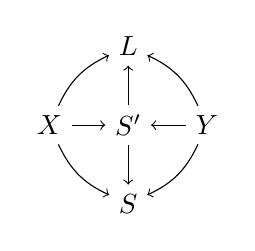
\begin{tikzpicture}
\node (a) at (0,1) {$L$};
\node (b) at (1,0) {$Y$};
\node (c) at (0,-1) {$S$};
\node (d) at (-1,0) {$X$};
\node (e) at (0,0) {$S'$};
%
\draw [<-] (a) edge[bend left=20] (b);
\draw [->] (b) edge[bend left=20] (c);
\draw [<-] (c) edge[bend left=20] (d);
\draw [->] (d) edge[bend left=20] (a);
\draw [<-] (a) edge (e);
\draw [->] (b) edge (e);
\draw [<-] (c) edge (e);
\draw [->] (d) edge (e);
\end{tikzpicture}
\]
\end{document}
